\chapter{Hardware}

As we introduced in \Cref{sec:background-pspin}, PsPIN is a RISC-V-based packet processing cluster implementing the sPIN in-network-computing paradigm.  However, PsPIN itself does not consist of a fully functional SmartNIC due to the lack of capability to receive and send packets; it also lacks an interface to read from and write to the system memory.  The following three classes of hardware components need to be implemented to achieve full functionality of a sPIN NIC: 

\begin{itemize}
    \item the \emph{data path}: the PsPIN cluster should be able to receive packet data from the network and (optionally) send a reply into the network;
    \item the \emph{control path}: the PsPIN cluster and other components should be configured from the host over various control registers and program memory (code and data); and finally,
    \item the \emph{host-side DMA}: the PsPIN cluster should be able to read from and write to the main memory on the host system to establish the full sPIN programming model.
\end{itemize}

An overview of all the hardware components is shown in \Cref{fig:hw-overview}.  We now walk through the design and implementation of these modules in more detail.

\begin{figure}
    \centering
    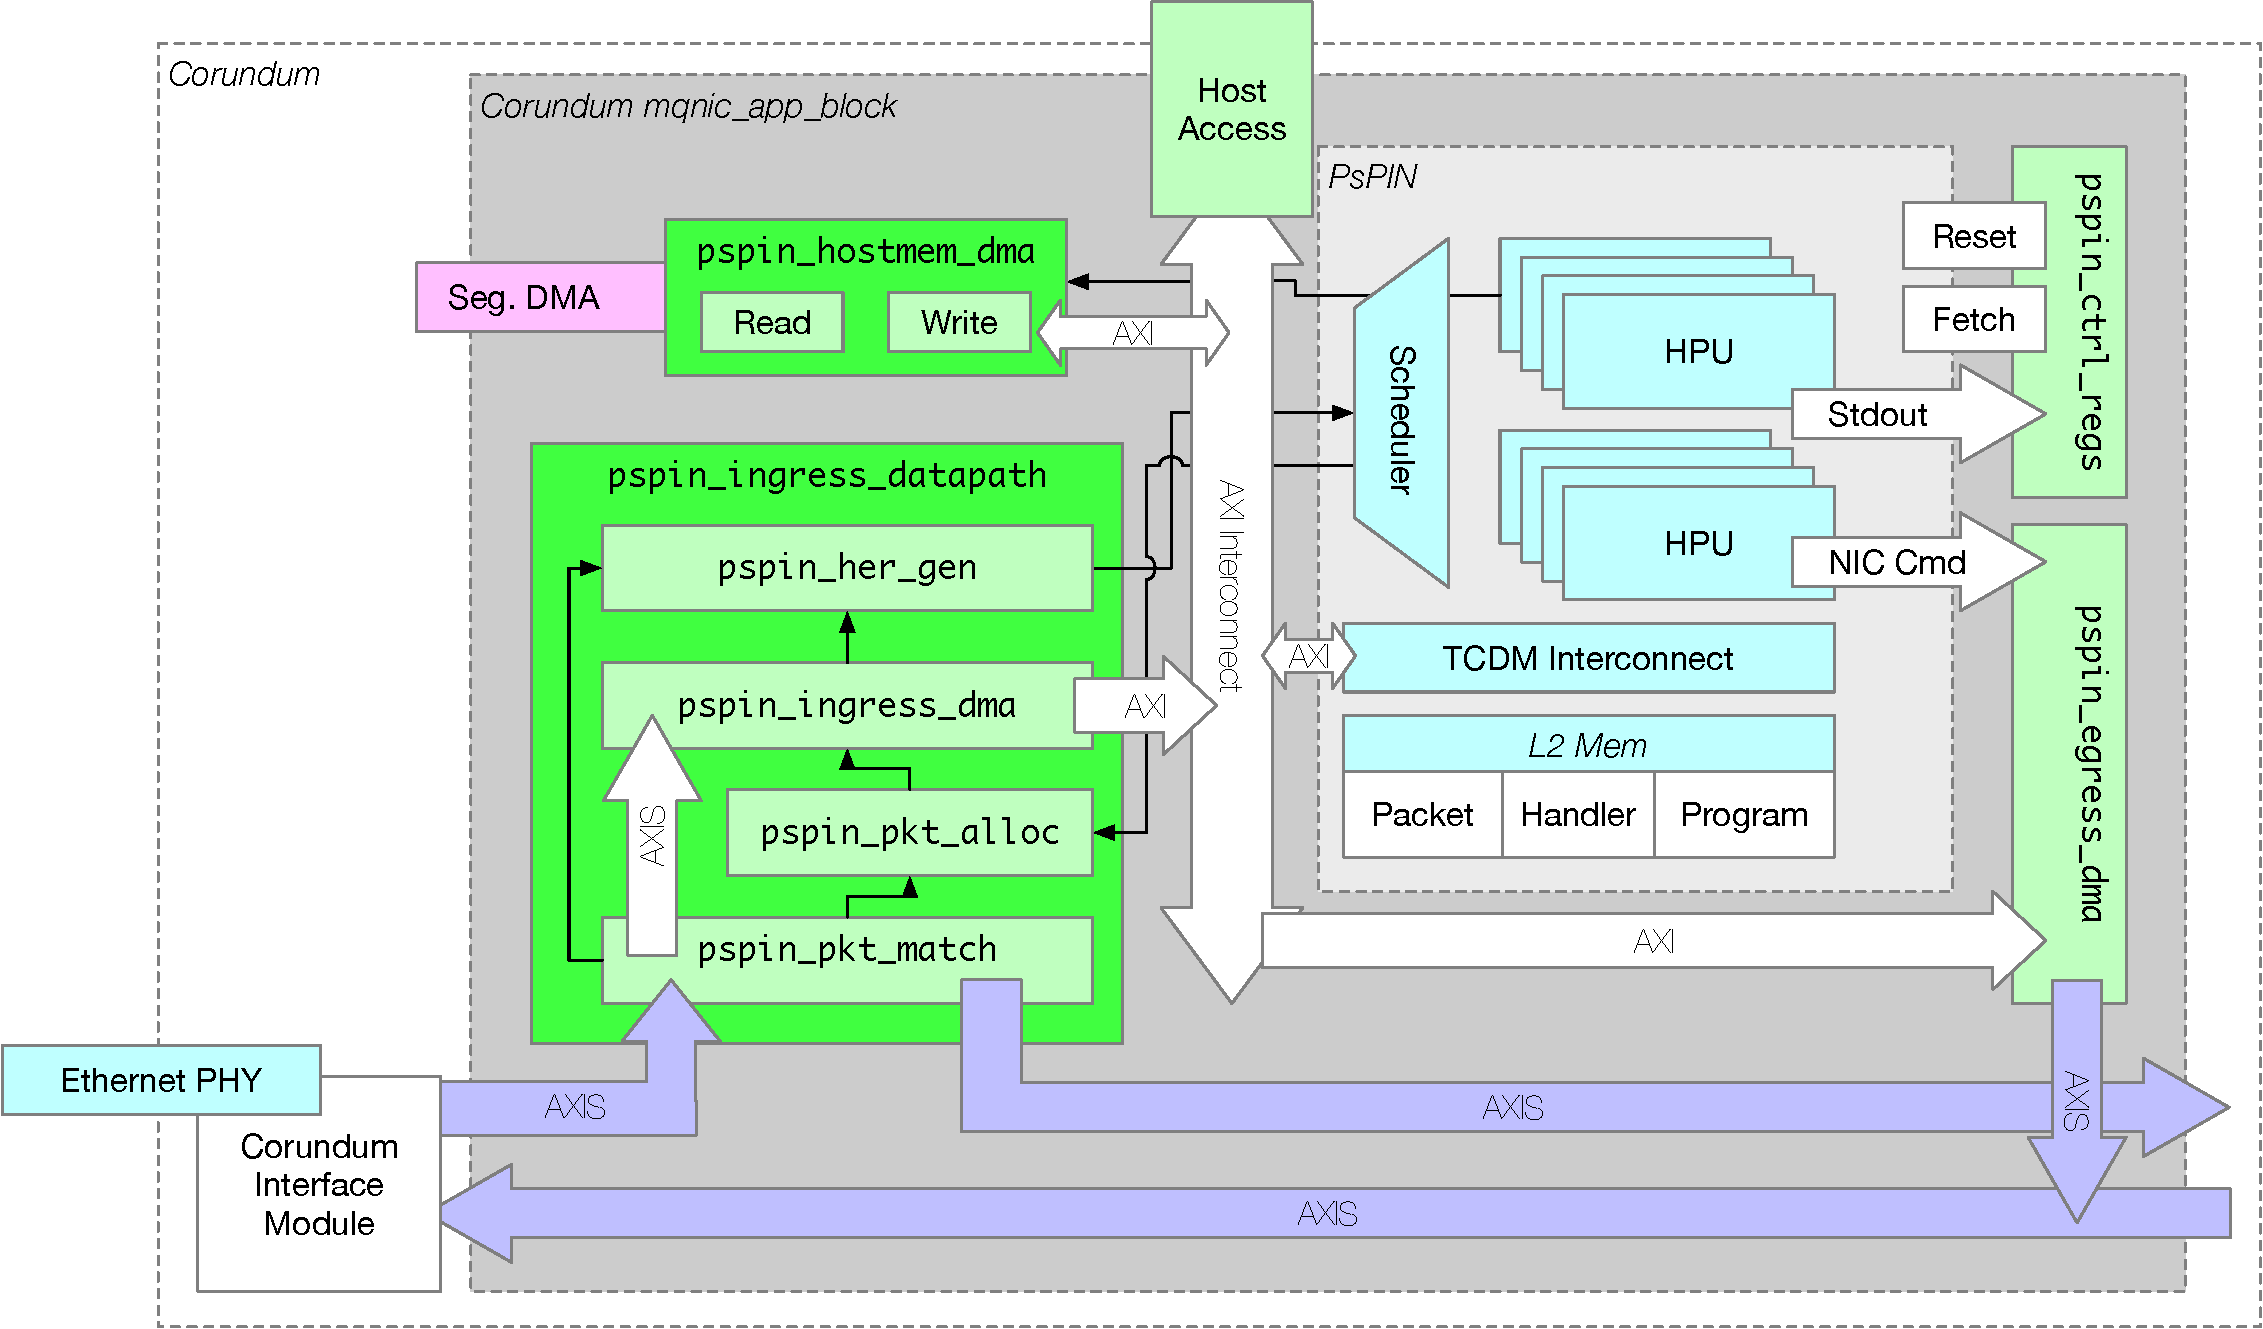
\includegraphics[width=\linewidth]{figures/hw-overview.pdf}
    \caption{Overview of the FPsPIN hardware.  Blocks marked in green are the modules implemented as part of this project to bridge the PsPIN cluster to Corundum.}
    \label{fig:hw-overview}
\end{figure}

\section{Control path}

The control path handles configuration of the PsPIN cluster as well as the various data path components \emph{before} the actual execution of handler code on the cluster.  There are three important control-path tasks to perform from the host, all of which are implemented over Corundum's slow-path 32-bit AXI-Lite interface with an address bus of 16 bits:

\begin{itemize}
    \item to toggle various control wires (e.g., reset, fetch enable, etc.) into the PsPIN cluster and datapath components;
    \item to read back standard output produced by PsPIN (i.e., \texttt{printf}); and
    \item to load program code and data onto memory in the PsPIN cluster.
\end{itemize}

\paragraph{Control wires} The control wires are configured through the \texttt{pspin\_ctrl\_regs} module.  The module exposes an AXI-Lite slave towards the AXI-Lite interconnect and converts this into simple \texttt{valid}-guarded interfaces for PsPIN and various datapath components to consume.  Some signal groups have requirements on \emph{consistency of update}, that is, the signals in the same group should always be consistent and no partial updates should be visible to the components being controlled.  Checks for this requirement happens in the kernel driver as we will introduce in \Cref{sec:sw-kmod}.  An overview of the exposed control signals from \texttt{pspin\_ctrl\_regs} is shown in \Cref{tab:ctrl-signals}.

\begin{table}[ht]
    \centering
    \begin{tabular}{lcl}
    \toprule
    Name & Direction & Description \\ \midrule
    \texttt{cl\_fetch\_en} & O & Fetch-enable control to PsPIN \\
    \texttt{aux\_rst} & O & Auxiliary reset for PsPIN and datapath \\
    \texttt{cl\_busy} & I & Cluster busy status from PsPIN \\
    \texttt{mpq\_full} & I & MPQ full status bitmap \\
    \texttt{match\_*} & O & Matching engine configuration \\
    \texttt{her\_gen\_*} & O & HER generator configuration \\
    \texttt{stdout\_*} & O & Standard output readback \\
    \bottomrule
    \end{tabular}
    \caption{Overview of the control wires consumed by \texttt{pspin\_ctrl\_regs}.  The configuration for the matching engine, HER generator, and standard output readback are described in the coming sections.}
    \label{tab:ctrl-signals}
\end{table}

\paragraph{Standard output access} To facilitate debugging of handler code on the PsPIN cluster, we implement a readback mechanism for the characters printed by the RISC-V cores.  The core executes \texttt{putchar} to write characters into the \texttt{apb\_stdout} module.  Different cores write to separate addresses exported by the module, allowing the module to demultiplex the incoming characters.  The module enqueues the characters toegether with the source core ID in a FIFO.  The FIFO is then read out from \texttt{pspin\_ctrl\_regs}.  To avoid introducing module ports on all levels of RTL hierarchy, we utilise the \emph{hierarchical reference scope}\footnote{\url{https://www.chipverify.com/verilog/verilog-hierarchical-reference-scope}} feature of Verilog to connect the output ports from \texttt{apb\_stdout} directly.  Finally, the host can read back the enqueued characters by reading out the \texttt{stdout\_*} registers through the register interface, demultiplex, and store the output as logs for future inspection.

\paragraph{Code and data download} The code and data of the packet handler program on PsPIN need to be loaded into the \emph{program memory} in PsPIN before we can start scheduling packets to execute on the HPUs.  The program memory is accessible through the \emph{host slave} port on the PsPIN cluster.  This port also allows write to the other two memory areas, the \emph{handler memory} and the \emph{packet memory}.  Together, this allows loading of compiled PsPIN program images onto the cluster memory.

We implement such access by connecting the upstream AXI-Lite port from Corundum, through a AXI-Lite interconnect and a AXI-Lite to AXI4 adpater, to the host slave port.  Note that the PsPIN address space on the host slave port is 32-bits.  However, we only have a 24-bit address space from the application block configuration port from Corundum.  Therefore, we perform a \emph{compression} in the address space by mapping the three memory areas closer together into the configuration port address space.  The loader in the userspace library, as later to be described in \Cref{sec:sw-lib}, will encode the PsPIN memory accesses according to this mapping.

\section{Data path}

Corundum provides access to raw Ethernet frames over the AXI Stream interface.  Three attachment points are available to the application block for reading ingress Ethernet frames out, as well as injecting egress frames:

\begin{itemize}
    \item \emph{Direct}: the AXI Stream interface directly after the Ethernet MACs and before most Corundum modules.  The interfaces are synchronous to the MAC clock (322.265625 MHz for 100 Gbps Ethernet).  This offers the lowest possible latency from the application block.
    \item \emph{Sync}: the AXI Stream interface after the CDC (clock domain crossing) FIFO for each port.  These interfaces are synchronous to the Corundum core clock (250 MHz).  They offer comparatively low latency.
    \item \emph{Interface}: the AXI Stream interface after the main packet aggregation FIFO per interface.  These interfaces are per interface (instead of per port; for example a 100 Gbps interface could be split into 4 25 Gbps ports) and are the simplest to process.  They are synchronous to the Corundum core clock (250 MHz).
\end{itemize}

The FPGA board we use, as described in \Cref{sec:eval-setup}, has two 100 Gbps interfaces; each interface can be further split up into 4 25 Gbps ports.  For simplicity of implementation, we attach the PsPIN datapath at the \emph{interface} attach point, such that we don't have to multiplex traffic from different ports by ourselves.

\subsection{Ingress}

After a packet has arrived at the \emph{interface} attach point, multiple tasks need to be done for an ingress packet before it lands in PsPIN memory and is ready for processing.  We implement four separate functional blocks as follows; together they form the ingress datapath module (\texttt{pspin\_ingress\_datapath}):

\begin{enumerate}
    \item \texttt{pspin\_\-pkt\_\-match}: match if the packet is to be processed by the SmartNIC cluster or to be forwarded to the normal Corundum datapath;
    \item \texttt{pspin\_\-pkt\_\-alloc}: allocate buffer for the incoming packet in the L2 packet buffer, free the buffer once it finishes processing;
    \item \texttt{pspin\_\-ingress\_\-dma}: DMA write the packet data into the L2 packet buffer
    \item \texttt{pspin\_\-her\_\-gen}: generate the Handler Execution Request to the PsPIN cluster
\end{enumerate}

We explain in detail the design 

\subsection{Egress}

On the egress path, \texttt{pspin\_egress\_dma} handles DMA read from the packet buffer to inject into the outbound AXI Stream of Corundum.  All these modules are controllable on the host through the control registers module \texttt{pspin\_ctrl\_regs}.

\section{Host DMA}

As defined in the sPIN specification, packet handlers running on PsPIN can read from or write to host memory.  This is enabled through the \texttt{pspin\_hostmem\_dma} module, which bridges the AXI master port of the PsPIN cluster to the segmented DMA interface\footnote{\url{https://github.com/corundum/verilog-pcie}} of Corundum.  We utilize the existing AXI Stream DMA client provided by Corundum and convert the output AXI Stream bus to AXI4 channels.  A notable limitation is that the adapter is not fully AXI-compliant (e.g., not supporting narrow bursts, etc.), which is acceptable as the bus master in PsPIN does not issue such requests.

\pengcheng{unaligned transfers: recover address from AXI burst wstrb}

\section{Design Considerations}
\pengcheng{PsPIN critical path analysis and why it could only run at 40 MHz}
\pengcheng{Cross clk domain considerations}

For the scope of this thesis, we adopt the approach of the \emph{simplest} hardware implementation possible.  This means that all modules are simple state machines without concurrency. This would not be an issue as of now as later discussed in \Cref{sec:hw-latency-analysis}. We implement all modules in Verilog.